\documentclass{article}
\title{Analiza algorytmów. Lista 4}
\author{Piotr Berezowski, 236749}

\usepackage{polski}
\usepackage[utf8]{inputenc}
\usepackage{enumerate}
% \usepackage{subfig}
\usepackage{amsmath}
\usepackage{amsfonts}
\usepackage{cleveref}
\usepackage{cases}
\usepackage{mathtools}
\usepackage{float}
\usepackage{graphicx}
\usepackage{caption}
\usepackage{subcaption}
\usepackage[ruled,vlined,linesnumbered,longend]{algorithm2e}
\graphicspath{ {./src/} }

\newenvironment{pseudokod}[1][htb]{
	\renewcommand{\algorithmcfname}{}
	\begin{algorithm}[#1]%
	}{
\end{algorithm}
}

\begin{document}
	\maketitle
	\pagenumbering{gobble}
	\newpage
    \pagenumbering{arabic}
    
    \section{Implementacja zadań}
    Implementacja zadania została wykonana w języku \textit{Julia} w wersji 1.4.1. Do uruchomienia skryptu z zadaniem wymagane jest doinstalowanie 
    pakietu \textit{Plots} odpowiedzialnego za rysowanie wykresów. 
    
    Załączone pliki:
        \begin{itemize}
            \item \textit{zad11.jl} - zawiera implementację symulatora dla podpunktu b zadania, funkcje obliczające $P(n,q)$ oraz funkcje rysujące wykresy.
        \end{itemize}

    Uruchomienie skryptu poleceniem \textit{julia zad11.jl} powinno stworzyć pliki zawierające wszystkie wykresy przedstawione w sprawozadniu.
	
	\section{Zadanie 11}
	\subsection{Opis zadania}

    Przeczytaj notatki do wykładu. Niech $0 < q < 1/2$ oznacza prawdopodobieństwo wydobycia kolejnego bloku przez adwersarza odpowiadające części
    mocy obliczeniowej będącej w jego posiadaniu. Niech $n$ oznacza liczbę potwierdzeń (nadbudowanych bloków) potrzebnych by uznać transakcję za 
    potwierdzoną. Niech $P(n,q)$ oznacza prawdopodobieństwo, że adwersarz o mocy $q$ będzie dysponował łańcuchem bloków równym lub dłuższym niż 
    ten budowany przez uczciwych użytkowników w momencie, gdy nadbudowali oni blok zawierający rozważaną transakcję $n$ blokami lub kiedykolwiek 
    później.
    \begin{itemize}
        \item Porównaj formuły na $P(n,q)$ uzyskane przez Nakamato i Grunspana. W szczególności:
        \begin{itemize}
            \item ustal $n= 1,3,6,12,24,48$ i przedstaw wykresy $P(n,q)$ w zależności od wartości $q$,
            \item ustal dopuszczalne prawd. sukcesu adwersarza $P(n,q) = 0.1\%,1\%,10\%$ i narysuj wykresy przedstawiające jak należy dobrać 
                wartość $n$ w zależności od wartości $q$.
        \end{itemize}
        \item Zaimplementuj symulator ataku „double spending”, który umożliwi eksperymentalne przybliżenie prawdopodobieństwa zdarzenia $P(n,q)$ 
            w zależności od wartościni $q$. Wskazówka: zaprojektuj eksperyment i powtórz go wielokrotnie (Metoda Monte Carlo). W raporcie starannie
            i dokładnie opisz ideę działania i kod symulatora.
        \item Porównaj wyniki symulatora do wyników analitycznych (wykresy). Jeśli pojawią się rozbieżności postaraj się je wyjaśnić.
    \end{itemize}
    
    \subsection{Rozwiązanie}

    \subsubsection{Porównanie formuł uzyskanych przez Nakamoto i Grunspana dla poszczególnych wartości $n$}

        \begin{figure}[H]
            % \centering
            \begin{subfigure}{0.6\textwidth}
                \centering
                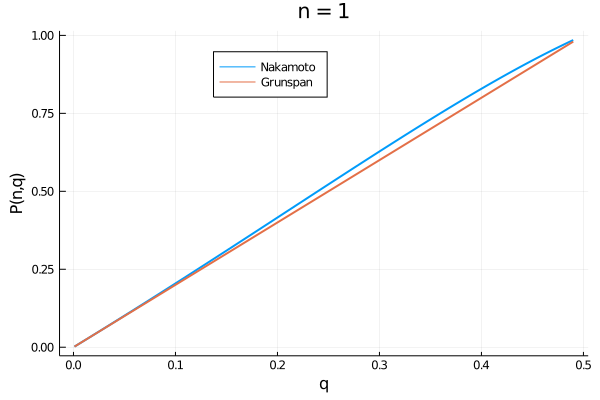
\includegraphics[width=\linewidth]{img/n=1.png}
                \caption{n = 1}
            \end{subfigure}
            \begin{subfigure}{0.6\textwidth}
                \centering
                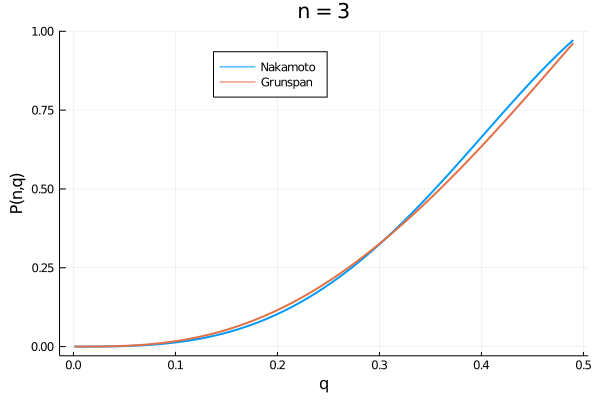
\includegraphics[width=\linewidth]{img/n=3.png}
                \caption{n = 3}
            \end{subfigure}
        % \end{figure}
        % \begin{figure}[H]
            \begin{subfigure}{0.6\textwidth}
                \centering
                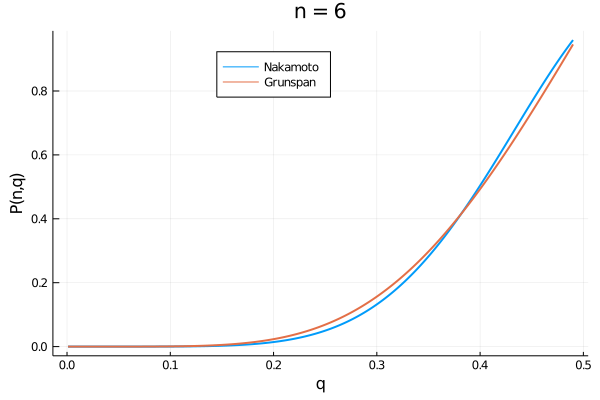
\includegraphics[width=\linewidth]{img/n=6.png}
                \caption{n = 6}
            \end{subfigure}
            \begin{subfigure}{0.6\textwidth}
                \centering
                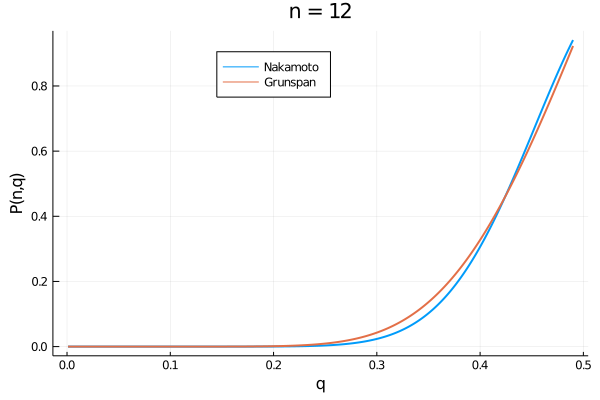
\includegraphics[width=\linewidth]{img/n=12.png}
                \caption{n = 12}
            \end{subfigure}
        % \end{figure}
        % \begin{figure}[H]
            \begin{subfigure}{0.6\textwidth}
                \centering
                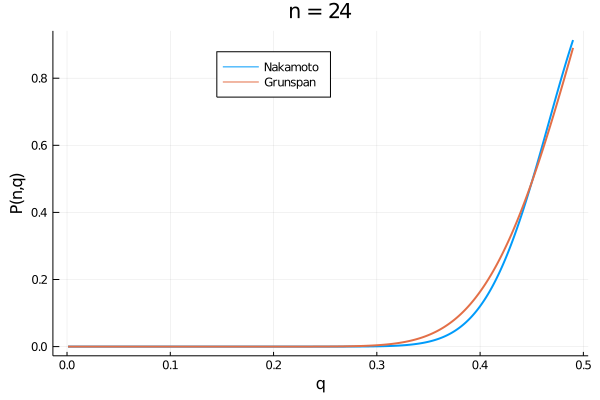
\includegraphics[width=\linewidth]{img/n=24.png}
                \caption{n = 24}
            \end{subfigure}
            \begin{subfigure}{0.6\textwidth}
                \centering
                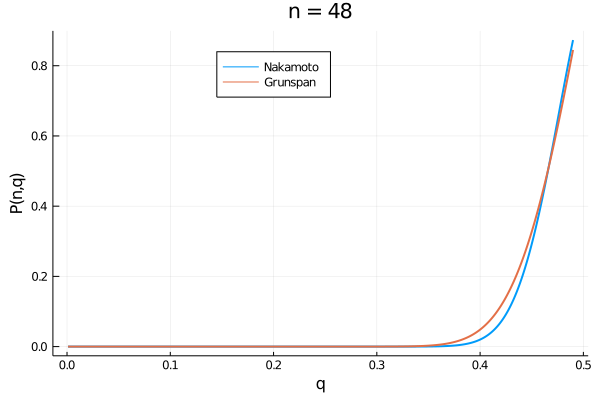
\includegraphics[width=\linewidth]{img/n=48.png}
                \caption{n = 48}
            \end{subfigure}
            \caption{$P(n,q)$ w zależności od $q$ dla różnych wartości $n$.}
        \end{figure}
    

    \subsubsection{Porównanie wartości $n$ spełniających dopuszczalną wartość $P(n,q)$ obliczaną przez obie formuły.}

        \begin{figure}[H]
            \centering
            \begin{subfigure}{0.65\textwidth}
                % \centering
                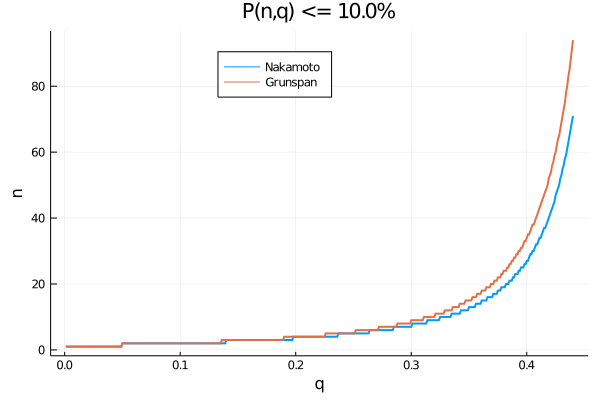
\includegraphics[width=\linewidth]{img/limit=0.1.png}
                \caption{$P(n,q) \leq 10\%$}
            \end{subfigure}

            \begin{subfigure}{0.65\textwidth}
                % \centering
                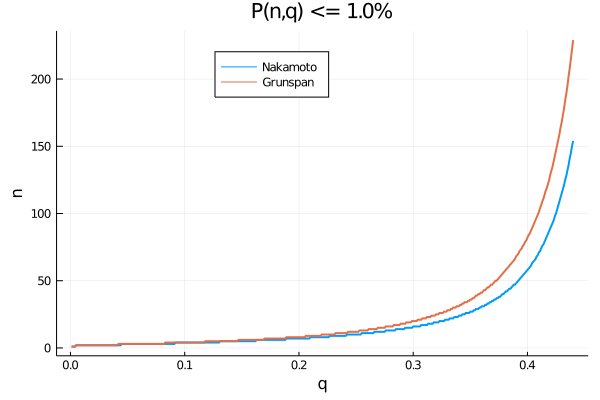
\includegraphics[width=\linewidth]{img/limit=0.01.png}
                \caption{$P(n,q) \leq 1\%$}
            \end{subfigure}

            \begin{subfigure}{0.65\textwidth}
                % \centering
                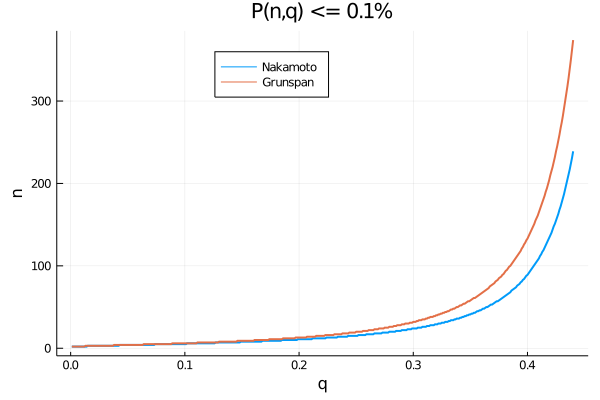
\includegraphics[width=\linewidth]{img/limit=0.001.png}
                \caption{$P(n,q) \leq 0.1\%$}
            \end{subfigure}

            \caption{Wartość $n$ w zależności od $q$ dla różnych dopuszczalnych wartości $P(n,q)$.}
        \end{figure}
 
    
    \subsection{Symulator ataku „double spending”}


    \begin{pseudokod}[H]
        \caption{doubleSpendingSimulation($n, q$)}
        \SetKwInOut{Input}{Input}
        \SetKwInOut{Output}{Output}
        \Input{$n$, $q$}
        \Output{$P(n,q)$ - prawdopodobieństwa zrównania się gałęzi adwersarza z najdłuższą}
        \BlankLine
        $advBlocks \gets 0$\;
        $usrBlocks \gets 0$\;
        \While{$usrBlocks < n$} {
            $r \gets rand( [0,1) )$\;
            \If{$r < q$} {
                $advBlocks \gets advBlocks + 1$\;
            }
            \Else {
                $usrBlocks \gets usrBlocks + 1$\;
            }
        }
        \BlankLine
        \If{$advBlocks \geq usrBlocks$} {
            \Return{$1$}
        }
        \Else {
            \Return{$(\frac{q}{1-q})^{usrBlocks-advBlocks}$}
        }
    \end{pseudokod}

    Powyższy pseudokod pokazuje w jaki sposób został zaimplementowany symulator ataku „double spending”. 
    
    Sytuacja początkowa prezentuje się 
    w ten sposób, że adwersarz zaczyna budować własną gałąź łańcucha zaczynając od ostatniego bloku najdłuższego istniejącego łańcucha. 
    W takiej sytuacji początkowa długość nowej „uczciwej” gałęzi jak i gałęzi adwersarza jest równa $0$. Następnie, dopóki gałąź uczciwych 
    użytkowników nie osiągnie długości $n$, obie gałęzie budowane są w następujący sposób:
    \begin{itemize}
        \item losujemy liczbę z zakresu $[0, 1)$
        \item jeśli wylosowana liczba jest mniejsza niż $q$ wydłużamy gałąź adwersarza
        \item w przeciwnym wypadku wydłużamy gałąź uczciwych użytkowników 
    \end{itemize}
    Kiedy długość gałęzi uczciwych użytkowników osiągnie długość równą $n$ znajdujemy się w jednej z dwóch sytuacji:
    \begin{itemize}
        \item gałąź adwersarza jest dłuższa niż $n$ - w tym przypadku zwracamy $1$, ponieważ zdarzenie zostało spełnione
        \item gałąź adwersarza jest krótsza niż $n$ i ma długość $k$ - w tym przypadku zwracamy prawdopodobieństwo zrównania się gałęzi 
            adwersarza z gałęzią uczciwych użytkowników równe $(\frac{q}{p})^{n-k}$
    \end{itemize}


    \subsection{Porównanie wyników symulatora i wyników analitycznych}

        \begin{figure}[H]
            \centering
            \begin{subfigure}{0.65\textwidth}
                % \centering
                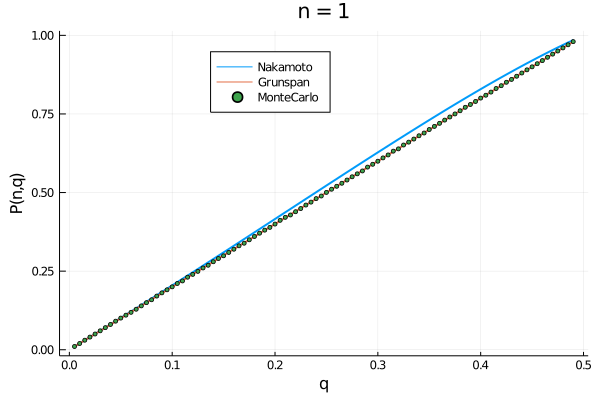
\includegraphics[width=\linewidth]{img/mc_n=1.png}
                \caption{$P(n,q)$ otrzymane z symulacji w porównaniu do formuł Nakamoto i Grunspana.}
            \end{subfigure}
    
            \begin{subfigure}{0.65\textwidth}
                % \centering
                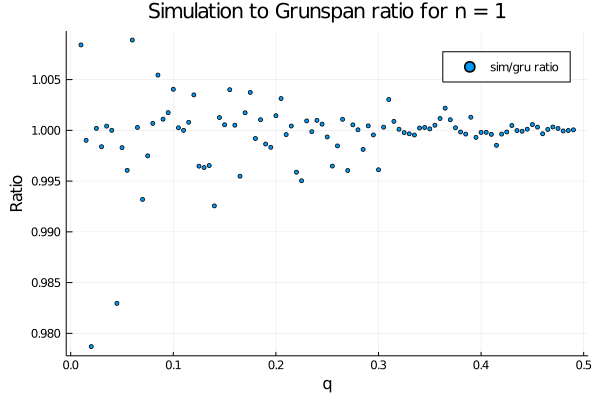
\includegraphics[width=\linewidth]{img/mc_to_gr_n=1.png}
                \caption{Stosunek $P(n,q)$ otrzymanego w symulacji do formuły Grunspana.}
            \end{subfigure}
    
            \begin{subfigure}{0.65\textwidth}
                % \centering
                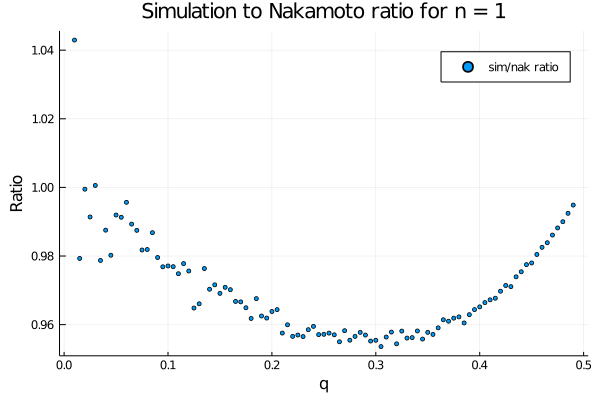
\includegraphics[width=\linewidth]{img/mc_to_na_n=1.png}
                \caption{Stosunek $P(n,q)$ otrzymanego w symulacji do formuły Nakamato.}
            \end{subfigure}
    
            \caption{Wyniki dla wartości $n = 1$}
        \end{figure}


        \begin{figure}[H]
            \centering
            \begin{subfigure}{0.65\textwidth}
                % \centering
                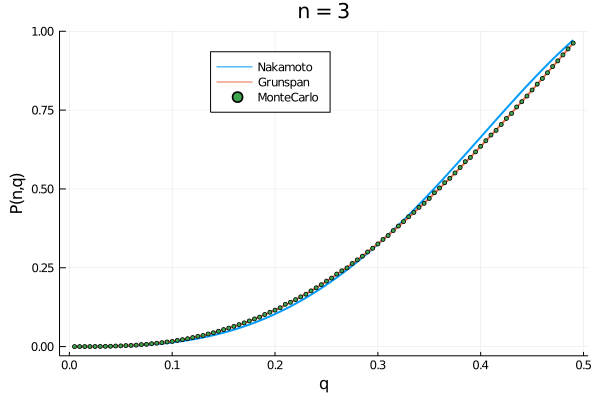
\includegraphics[width=\linewidth]{img/mc_n=3.png}
                \caption{$P(n,q)$ otrzymane z symulacji w porównaniu do formuł Nakamoto i Grunspana.}
            \end{subfigure}
    
            \begin{subfigure}{0.65\textwidth}
                % \centering
                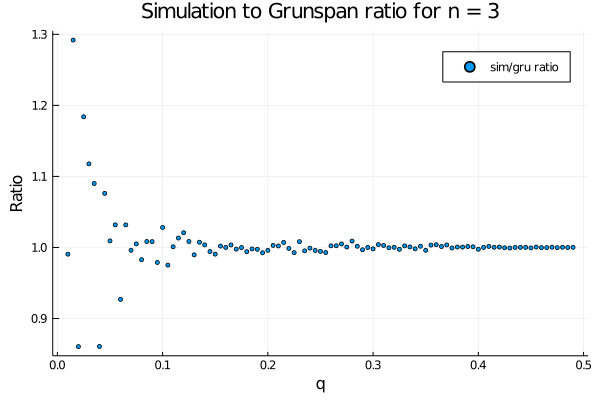
\includegraphics[width=\linewidth]{img/mc_to_gr_n=3.png}
                \caption{Stosunek $P(n,q)$ otrzymanego w symulacji do formuły Grunspana.}
            \end{subfigure}
    
            \begin{subfigure}{0.65\textwidth}
                % \centering
                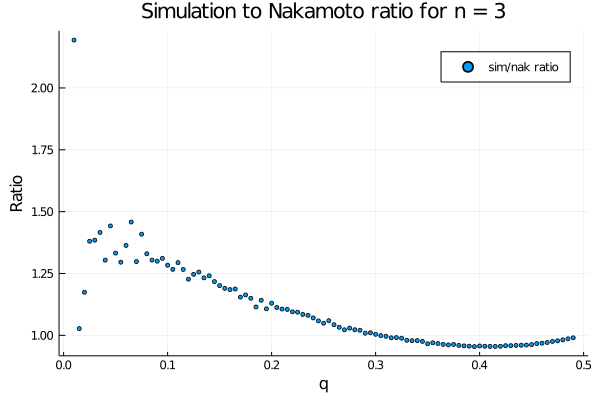
\includegraphics[width=\linewidth]{img/mc_to_na_n=3.png}
                \caption{Stosunek $P(n,q)$ otrzymanego w symulacji do formuły Nakamato.}
            \end{subfigure}
    
            \caption{Wyniki dla wartości $n = 3$}
        \end{figure}


        \begin{figure}[H]
            \centering
            \begin{subfigure}{0.65\textwidth}
                % \centering
                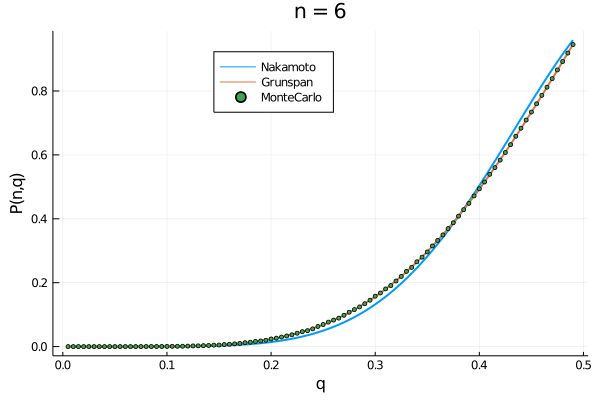
\includegraphics[width=\linewidth]{img/mc_n=6.png}
                \caption{$P(n,q)$ otrzymane z symulacji w porównaniu do formuł Nakamoto i Grunspana.}
            \end{subfigure}
    
            \begin{subfigure}{0.65\textwidth}
                % \centering
                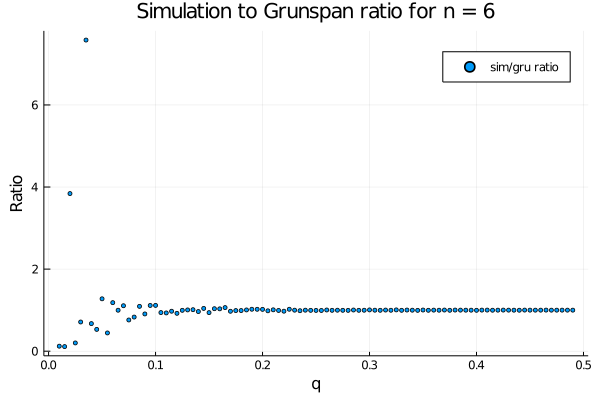
\includegraphics[width=\linewidth]{img/mc_to_gr_n=6.png}
                \caption{Stosunek $P(n,q)$ otrzymanego w symulacji do formuły Grunspana.}
            \end{subfigure}
    
            \begin{subfigure}{0.65\textwidth}
                % \centering
                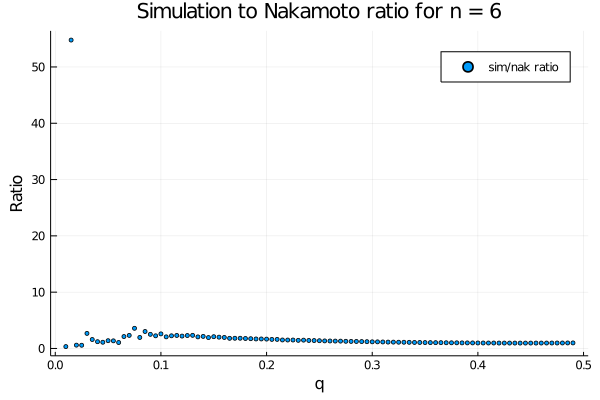
\includegraphics[width=\linewidth]{img/mc_to_na_n=6.png}
                \caption{Stosunek $P(n,q)$ otrzymanego w symulacji do formuły Nakamato.}
            \end{subfigure}
    
            \caption{Wyniki dla wartości $n = 6$}
        \end{figure}


        \begin{figure}[H]
            \centering
            \begin{subfigure}{0.65\textwidth}
                % \centering
                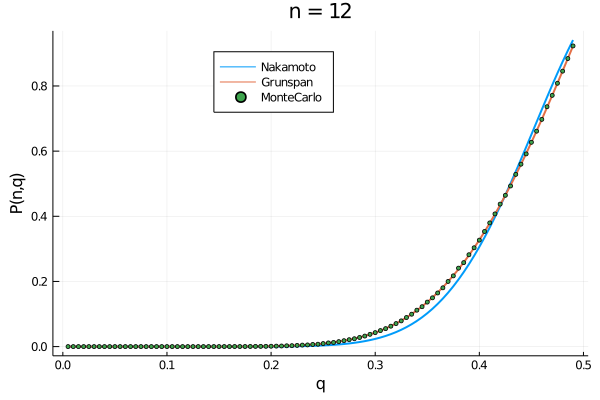
\includegraphics[width=\linewidth]{img/mc_n=12.png}
                \caption{$P(n,q)$ otrzymane z symulacji w porównaniu do formuł Nakamoto i Grunspana.}
            \end{subfigure}
    
            \begin{subfigure}{0.65\textwidth}
                % \centering
                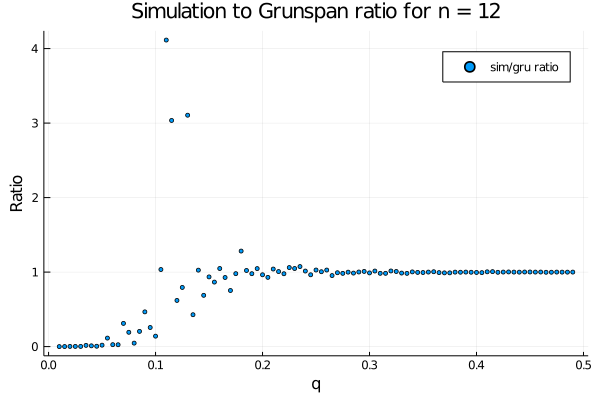
\includegraphics[width=\linewidth]{img/mc_to_gr_n=12.png}
                \caption{Stosunek $P(n,q)$ otrzymanego w symulacji do formuły Grunspana.}
            \end{subfigure}
    
            \begin{subfigure}{0.65\textwidth}
                % \centering
                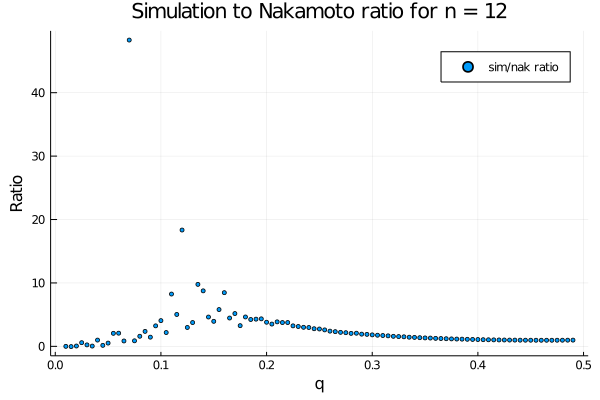
\includegraphics[width=\linewidth]{img/mc_to_na_n=12.png}
                \caption{Stosunek $P(n,q)$ otrzymanego w symulacji do formuły Nakamato.}
            \end{subfigure}
    
            \caption{Wyniki dla wartości $n = 12$}
        \end{figure}


        \begin{figure}[H]
            \centering
            \begin{subfigure}{0.65\textwidth}
                % \centering
                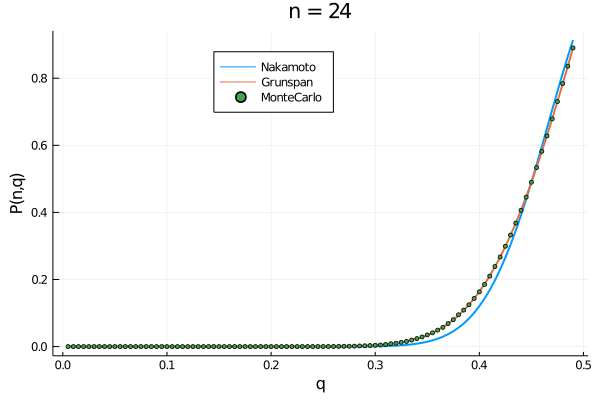
\includegraphics[width=\linewidth]{img/mc_n=24.png}
                \caption{$P(n,q)$ otrzymane z symulacji w porównaniu do formuł Nakamoto i Grunspana.}
            \end{subfigure}
    
            \begin{subfigure}{0.65\textwidth}
                % \centering
                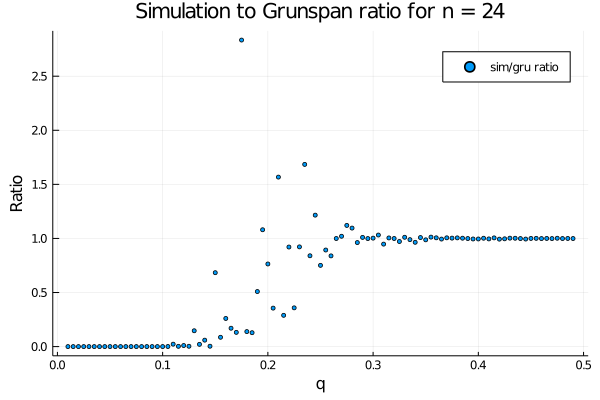
\includegraphics[width=\linewidth]{img/mc_to_gr_n=24.png}
                \caption{Stosunek $P(n,q)$ otrzymanego w symulacji do formuły Grunspana.}
            \end{subfigure}
    
            \begin{subfigure}{0.65\textwidth}
                % \centering
                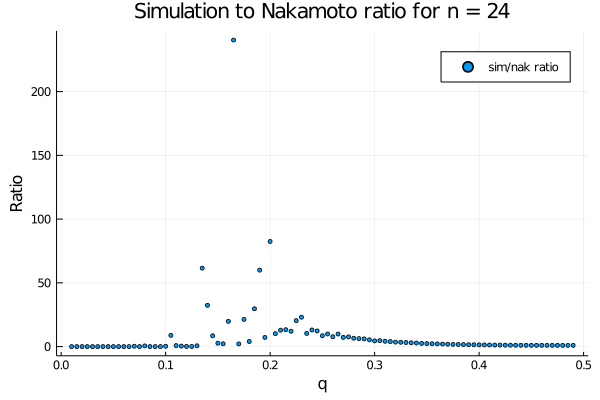
\includegraphics[width=\linewidth]{img/mc_to_na_n=24.png}
                \caption{Stosunek $P(n,q)$ otrzymanego w symulacji do formuły Nakamato.}
            \end{subfigure}
    
            \caption{Wyniki dla wartości $n = 24$}
        \end{figure}


        \begin{figure}[H]
            \centering
            \begin{subfigure}{0.65\textwidth}
                % \centering
                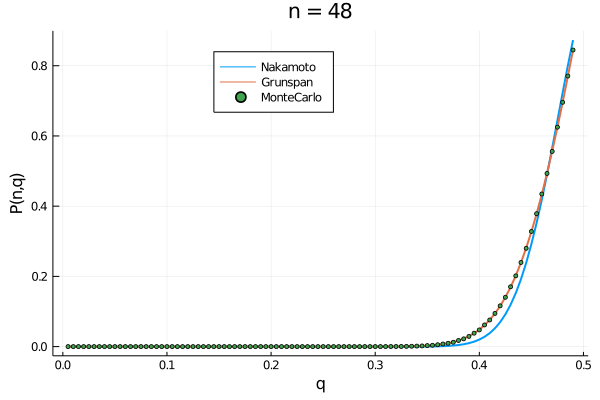
\includegraphics[width=\linewidth]{img/mc_n=48.png}
                \caption{$P(n,q)$ otrzymane z symulacji w porównaniu do formuł Nakamoto i Grunspana.}
            \end{subfigure}
    
            \begin{subfigure}{0.65\textwidth}
                % \centering
                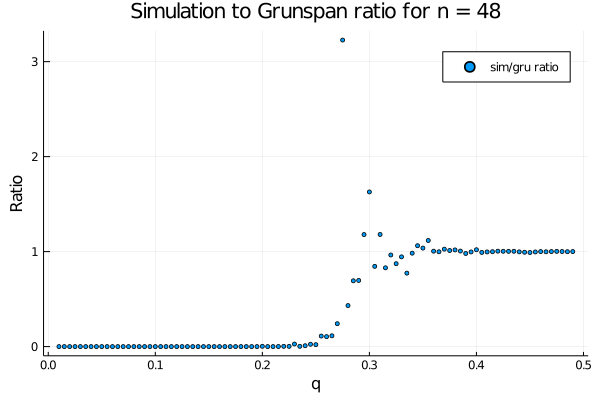
\includegraphics[width=\linewidth]{img/mc_to_gr_n=48.png}
                \caption{Stosunek $P(n,q)$ otrzymanego w symulacji do formuły Grunspana.}
            \end{subfigure}
    
            \begin{subfigure}{0.65\textwidth}
                % \centering
                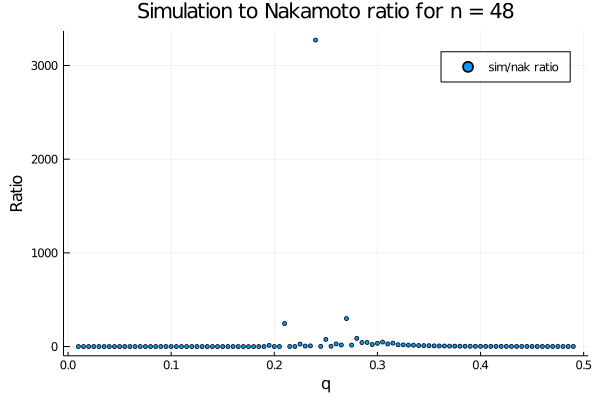
\includegraphics[width=\linewidth]{img/mc_to_na_n=48.png}
                \caption{Stosunek $P(n,q)$ otrzymanego w symulacji do formuły Nakamato.}
            \end{subfigure}
    
            \caption{Wyniki dla wartości $n = 48$}
        \end{figure}

        
    


\end{document}